\section{数的诞生}

\begin{frame}
	\begin{block}{你能想到那些简单的计数方式?}\pause
		\begin{itemize}[<+-| alert@+>]
			\item 绳子打结
			\item 骨头穿孔
			\item 泥板刻痕
			\item ……
		\end{itemize}
	\end{block}
\end{frame}

\begin{frame}\frametitle{最早的数字}
	\begin{columns}[c]
		\begin{column}{0.6\textwidth}
			\begin{question}
				最早的数字出现在什么时候?\\
				\begin{enumerate}[(A)]
					\item 十万年前
					\item 三万年前
					\item 一万年前
					\item 五千年前
				\end{enumerate}
			\end{question}\pause
			\begin{answer}
				(B)\\
				数的第一次使用可以追溯到大约公元三万年前,迄今为止发现的最早的例子是在南非的一个洞穴里。
			\end{answer}\pause
		\end{column}
	\begin{column}{0.3\textwidth}
		\begin{figure}
			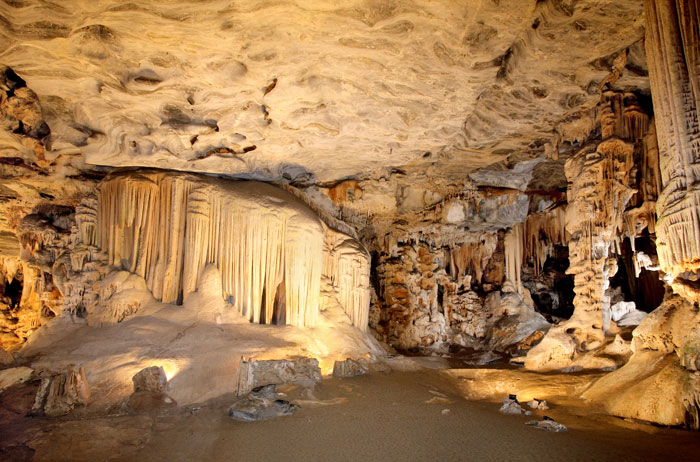
\includegraphics[width=\textwidth]{cango_cave_1.jpg}\\
			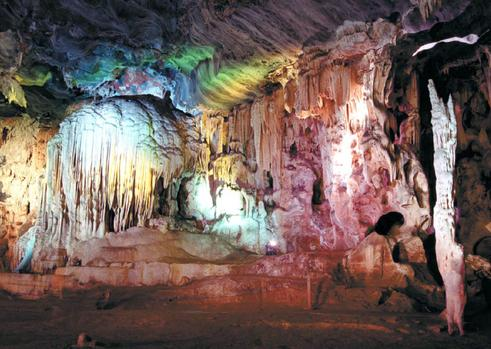
\includegraphics[width=\textwidth]{cango_cave_2.jpg}
			\caption{南非·甘果洞}
		\end{figure}
	\end{column}
	\end{columns}
\end{frame}

\begin{frame}{一则笑话}
	\begin{block}{谁说出的数字大?}\pause
	{
		两个匈牙利贵族决定做一次数数游戏——谁说出的数字最大谁赢。\\
		``好,''一个贵族说,``你先说把!''\\
		另一个绞尽脑汁想了好久,终于说出他所想到的最大数字:``3''。\\
		现在轮到第一个动脑筋了。苦思冥想了更久,他表示弃权说:``你赢啦!''\\
		\rightline{——伽莫夫《从一到无穷大》}
	}
	\end{block}\pause
	\begin{question}
		最大的数是多少?
	\end{question}
\end{frame}